\documentclass[12pt,letterpaper,addpoints]{exam}
\usepackage[utf8]{inputenc}
\usepackage{amsmath}
\usepackage{amsfonts}
\usepackage{amssymb}
\usepackage{amsthm}
\usepackage{graphicx}
\usepackage{tabularx}
\usepackage[left=2cm,right=2cm,top=2cm,bottom=2cm]{geometry}
\usepackage{multicol}
\usepackage{multirow,array}
\usepackage{newtxtext,newtxmath}
\usepackage{lastpage}
\usepackage{enumitem}
\usepackage{pdfpages}
\newcolumntype{Y}{>{\centering\arraybackslash}X}
\firstpageheader{}{}{
\includegraphics[scale=0.5]{BHCClogoBW.jpg}\hspace{-40pt}\vspace{-50pt}}
\firstpagefooter{}{}{Page \thepage ~of \pageref{LastPage}}
\runningheader{ \textsc{Math 181 2nd Exam}}{}{ \textsc{Spring 2019}}%{
\includegraphics[scale=.5]{BHCClogoBW.jpg}\vspace{-10pt}}%\hspace{-60pt}\vspace{-10pt}}
\runningheadrule
\runningfooter{}{}{Page \thepage ~of \pageref{LastPage}}
\renewcommand{\thequestion}{{\bf Q\arabic{question}}}
%\renewcommand{\questionlabel}{{\thequestion .}}
%\pointformat{\fbox{\themarginpoints \,pt}}
%\pointsinrightmargin
%\setlength{\rightpointsmargin}{1.5cm}
%\pointsinmargin
%\setlength{\marginpointssep}{10pt}

\begin{document}

\newcommand{\AND}{~\textsc{and}~}
\newcommand{\OR}{~\textsc{or}~}

\begin{center}
\text{ }\\
\vspace{40pt}
\textsc{{\Huge Math 181 2nd Exam}}\\\vspace{5pt}
\textsc{{\large Spring 2019}}\\
\vspace{60pt}
\makebox[\textwidth]{\large Name:\enspace\hrulefill}\\
\vspace{40pt}
\fbox{\fbox{\begin{minipage}{6in}
\vspace{0.2in}
\begin{itemize}
\item Write your {\bf full name} on the line above.
\item Show your work. Incorrect answers with work can receive partial credit.
\item Attempt every question; showing you understand the question earns some credit.
\item If you run out of room for an answer, continue on the back of the page. Before doing so, write ``see back'' with a circle around it.
\item You can use 1 page (front and back) of notes in addition to the formula sheet (on page 2) and $z$-table (last page).
\item You can use (and probably need) a calculator.
\item You can use the Geogebra Scientific Calculator instead of a calculator. You need to put your phone on {\bf airplane mode} and then within the application, start {\bf exam mode}; you should see a green bar with a timer counting up.
\item If a question is confusing or ambiguous, please ask for clarification; however, you will not be told how to  answer the question.
\item {\bf Box your final answer}.
\item You can rip off the $z$-table, but please keep the rest of the test intact.
\vspace{0.2in}
\end{itemize}
\end{minipage}
\begin{minipage}{0.2in}\text{ }\end{minipage}}}
\vfill
Do not write in this grade table.\\
\gradetable[h][questions]\\
\vfill
\end{center}

%%%%%%%%%%%%%%%%%%%%%%%%%%%%%%%%%%%%%%%%%%%%%%%%%%%%%%%%%%%%%%%%%%%%%%%%%%%%%%%
\newcommand{\N}[2]{\mathcal{N}\big(#1\,,~#2\big)}
\newcommand{\Bern}[1]{\texttt{Bern}\big(#1\big)}
\newcommand{\Geo}[1]{\texttt{Geo}\big(#1\big)}
\newcommand{\B}[2]{\mathcal{B}\big(#1\,,~#2\big)}
\newcommand{\Sampp}[2]{\texttt{Samp}_{\hat{p}}\big(#1,~#2\big)}
%\newcommand{\Sampx}[2]{\texttt{Samp}_{\hat{p}}\big(#1,~#2\big)}

\newpage

\begin{multicols}{2}

%\rhead{\textsc{Definitions and Formulas}}

{\bf Normal Distribution:}\\
$X \sim \N{\mu}{\sigma}$\\
$\mu = \text{ population mean} $\\
$\sigma = \text{ population standard deviation} $\\
$x = \text{ possible value of }X $\\
$\ell = \text{ percentile of } x \text{ (left area)}$\\
$\Phi(z) = \text{ standard normal cumulative function}$
\begin{align*}
z &= \frac{x-\mu}{\sigma}\\
P(X < x) &= \Phi(z)\\
\ell &= \Phi(z)\\
z &= \Phi^{-1}(\ell)
\end{align*}

{\bf Bernoulli Distribution:}\\
$X \sim \Bern{p} $\\
$X = \text{ 0 for fail or 1 for success}$\\
$p = \text{ probability of success}$
\begin{align*}
P(X=0) ~&=~ 1-p \\
P(X=1) ~&=~ p \\
\mu ~&=~ p\\
\sigma ~&=~ \sqrt{p(1-p)}
\end{align*}

{\bf Geometric Distribution:}\\
$X \sim \Geo{p}$ \\
$X = \text{ number of trials until first success}$\\
$p = \text{ probability of success on each trial}$\\
$n = \text{ a possible number of trials}$
\begin{align*}
P(X=n) ~&=~ (1-p)^{n-1}(p)\\
\mu ~&=~ \frac{1}{p}\\
\sigma ~&=~ \sqrt{\frac{1-p}{p^2}} 
\end{align*}

{\bf Mean-Sampling Distribution:}\\
$\bar{X} = \text{ sample mean}$\\
$s = \text{ sample standard deviation}$\\
$n = \text{ sample size}$\\
$\mu = \text{ population mean}$\\
$\sigma = \text{ population standard deviation}$\\
$SE = \text{ standard error}$
$$SE = \frac{\sigma}{\sqrt{n}} $$
If $n\ge 30$ (or if population is normal) then:
$$\bar{X} \sim \N{\mu}{SE} $$

\columnbreak

{\bf Binomial Distribution:}\\
$X \sim \B{n}{p}$\\
$X = \text{ number of successes from $n$ trials} $\\
$p = \text{ probability of success on each trial}$\\
$n = \text{ number of trials}$\\
$k = \text{ a possible number of successes}$
\begin{align*}
P(X=k) ~&=~ {n \choose k} p^k (1-p)^{n-k}\\
\mu ~&=~ np\\
\sigma ~&=~ \sqrt{np(1-p)} 
\end{align*}
If $np \ge 10$ and $n(1-p) \ge 10$, then
$$X \sim \N{\mu}{\sigma} $$
Continuity correction:
$$P(X \le k) ~\approx~ \Phi\left(\frac{k+0.5-\mu}{\sigma}\right)$$

{\bf Confidence Interval:}\\
$CI = \text{ confidence interval}$\\
$\gamma = \text{ confidence level}$\\
$\bar{x} = \text{ sample mean}$ \\
$s = \text{ sample standard deviation}$ 
\begin{align*}
z^{\star} &= \Phi^{-1}\left(\frac{\gamma+1}{2} \right) \\
SE &\approx \frac{s}{\sqrt{n}}\\
CI &= \bar{x} \pm z^{\star} SE
\end{align*}

{\bf Hypothesis testing:}\\
$H_0:~~~\mu = \mu_0$\\
$H_A:~~~\mu \ne \mu_0$\\
$\bar{x} = \text{ a possible/specific/observed sample mean}$\\
$s = \text{ sample standard deviation}$\\
$\alpha = \text{ significance level} $
\begin{align*}
\sigma &\approx s\\
z &= \frac{\bar{x}-\mu_0}{SE}\\\\
p\text{-value } &= P\left(\lvert Z \rvert > |z|  \right)\\
&= 2 \cdot \Phi\left( -|z| \right)
\end{align*}
If $p$-value $< \alpha$, then reject $H_0$, else retain $H_0$.

\end{multicols}


\newpage
\printanswers
\newcommand{\zlo}{z_\textsc{lower}}
\newcommand{\zhi}{z_\textsc{upper}}


\begin{questions}
\question[10] Let random variable $X$ be normally distributed with mean $\mu=33$ and standard deviation $\sigma=4$.
\begin{parts}
\part Evaluate $P(X < 37)$.
\begin{solution}
We find a $z$-score.
$$z = \frac{37-33}{4} = 1 $$
We use the $z$ table to evaluate the probability.
$$P(X<37) ~=~ P(Z<1) ~=~ \Phi(1) ~=~ \fbox{0.8413} $$
\end{solution}
\vfill
\part Determine $x$ such that $P(X<x) = 0.33$.
\begin{solution}
We find the $z$-score from the $z$-table.
$$z ~=~ \Phi^{-1}(0.33) ~=~ -0.44 $$
We convert this $z$-score into an $x$-score.
\begin{align*}
x ~&=~ \mu+z\sigma \\
&=~ 33+(-0.44)(4) \\
&=~ \fbox{31.24}
\end{align*}
\end{solution}
\vfill
\end{parts}

\newpage


\question[10] Imagine a scratch-off lottery has a chance of success $p=0.01$.
\begin{parts}
\part What is the mean number of trials until the first success?
\begin{solution}
This situaton is described by a geometric distribution.
$$\mu ~=~ \frac{1}{p} ~=~ \frac{1}{0.01} ~=~ \fbox{100} $$
The mean number of trials is 100. The expected number of trials is 100.
\end{solution}
\vfill
\part What is the probability of getting the first success on the twelfth trial?
\begin{solution}
This situation is still described by a geometric distribution. So, we use the geometric probability formula: $P(X=n) ~&=~ (1-p)^{n-1}p$.
\begin{align*}
 \\
P(X=12) ~~&=~~ (1-0.01)^{12-1}(0.01) \\
&=~~ (0.99)^{11}(0.01) \\
&=~~ \fbox{0.00895}
\end{align*}
\end{solution}
\vfill
\end{parts}

\newpage


\question[10] Let each trial have a chance of success $p=0.25$. We will predict what happens when we have 100 trials.
\begin{parts}
\part What is the probability of getting exactly 26 successes?
\begin{solution}
This situation is described by a binomial distribution.
\begin{align*}
P(X=26) ~~&=~~ {100 \choose 26} (0.25)^{26}(0.75)^{74}\\
&=~~ \fbox{0.0883}
\end{align*}
\end{solution}
\vfill
\part What is the probability of getting fewer than 26 successes? (Use a normal approximation and continuity correction.)
\begin{solution}
We find the parameters needed to construct a normal approximation.
%\begin{align*}
%\mu ~~&=~~ np\\
%&=~~ (100)(0.25) \\
%&=~~ 25 
%\end{align*}
$$\mu ~~=~~ np ~~=~~ (100)(0.25) ~~=~~ 25$$
\begin{align*}
\sigma ~~&=~~ \sqrt{np(1-p)}\\
&=~~ \sqrt{(100)(0.26)(0.74)} \\
&=~~ 4.3863
\end{align*}
Here is a sketch:
\begin{center}
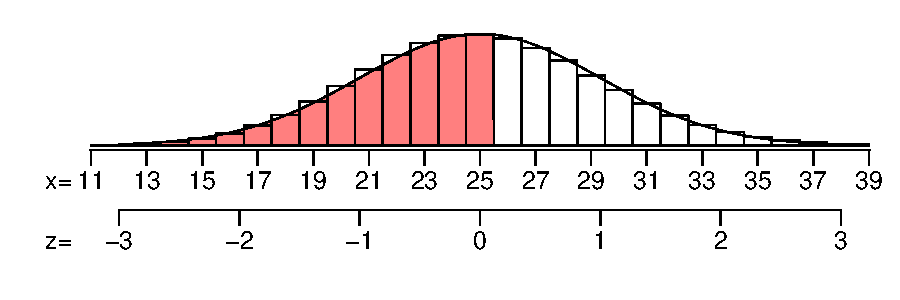
\includegraphics[scale=0.7]{figures/sketch12.pdf}
\end{center}
We find the $z$ score of the boundary.
$$z = \frac{25.5-25}{4.3863} = 0.11 $$
We calculate the probability.
$$P(X<26) ~=~ P(X<25.5) ~=~ P(Z<0.11) ~=~ \fbox{0.5438} $$
\end{solution}
\vfill
\part What is the probability of getting more than 26 successes? 
\begin{solution}
The easiest way to do this is by recognizing these three probabilities are mutually exclusive and exhaustive.
$$1-0.0883-0.5438 ~=~ \fbox{0.3679} $$
\end{solution}
\vfill
\end{parts}


\newpage


\question[10] A uniformly distributed population has a mean $\mu=250$ and a standard deviation $\sigma=18$. When a sample of size $n=144$ is taken, what is the probability of getting a sample mean between 247 and 253?
\begin{solution}
This situation is described by a mean-sampling distribution. We find the standard error.
$$SE ~~=~~ \frac{\sigma}{\sqrt{n}} ~~=~~ \frac{18}{\sqrt{144}} ~~=~~ 1.5$$
Even though the population is uniformly distributed, the sampling distribution is approximately normal.
$$\bar{X} \sim \N{250}{1.5} $$
We find the $z$-scores.
$$\zlo ~=~ \frac{247-250}{1.5} ~=~ -2$$
$$\zhi ~=~ \frac{253-250}{1.5} ~=~ 2$$
Here is a sketch:
\begin{center}
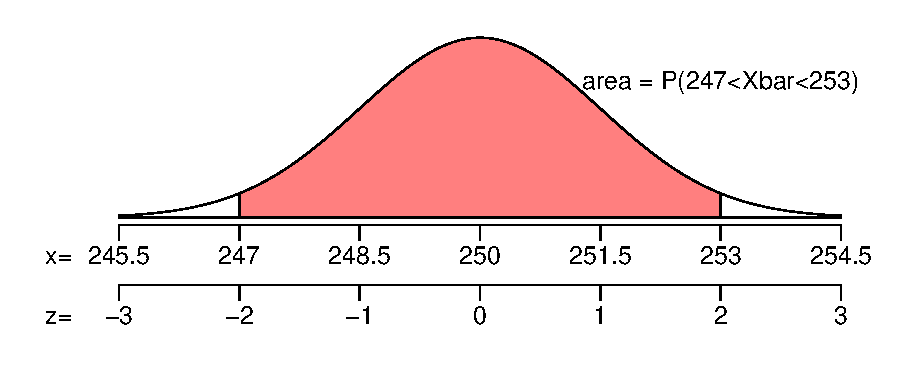
\includegraphics[scale=1]{figures/sketch13.pdf}
\end{center}
We find the probability.
\begin{align*}
P(247 < \bar{X} < 253) ~~&=~~ P(-2 < Z < 2)\\
&=~~ \Phi(2)-\Phi(-2) \\
&=~~ \fbox{0.9545}
\end{align*}
\end{solution}
\newpage


\question[10] A sample of size $n=144$ has a mean $\bar{x}=253.92$ and a standard deviation $s=17.54$. Construct a confidence interval of the population's mean based on the sample using a confidence level $\gamma=0.99$.
\begin{solution}
We find $z^\star$.
\begin{align*}
z^\star ~~&=~~ \Phi^{-1}\left(\frac{0.99+1}{2}\right) \\
&=~~ \Phi^{-1}(0.995) \\
&=~~ 2.58
\end{align*}
We find the standard error.
$$SE ~=~ \frac{17.54}{\sqrt{144}} ~=~ 1.4617 $$
We determine the confidence interval. (Old $\bar{x}$ on first print)
\begin{align*}
CI ~&=~ \bar{x} \pm z^\star SE \\
&=~ 254.87 \pm (2.58)(1.4617) \\
&=~ \fbox{\left(251.1\,,~258.6\right)}
\end{align*}
We determine the confidence interval. (Answer to updated problem.)
\begin{align*}
CI ~&=~ \bar{x} \pm z^\star SE \\
&=~ 253.92 \pm (2.58)(1.4617) \\
&=~ \fbox{\left(250.1\,,~257.7\right)}
\end{align*}
\end{solution}

\newpage


\question[10] Imagine you thought a uniformly distributed population had a mean $\mu=250$ and standard deviation $s=18$. However, you are skeptical, so you decide to run a two-tailed hypothesis test with a significance level $\alpha=0.01$.

Your sample of size $n=144$ results in a mean $\bar{x}=253.92$. 

\begin{parts}
\part State the hypotheses.
\begin{solution}
$$H_0: ~~\mu=250 $$
$$H_A: ~~\mu\ne 250 $$
\end{solution}
\vfill
\part Describe and sketch the null's sampling distribution. 
\begin{solution}
We need the standard error for a sampling distribution. 
$$SE = \frac{18}{\sqrt{144}} = 1.5 $$
We think the null's sampling distribution is normal with mean $\mu=250$ and standard deviation $\sigma=1.5$.
$$\bar{X} \sim \N{250}{1.5} $$
\begin{center}
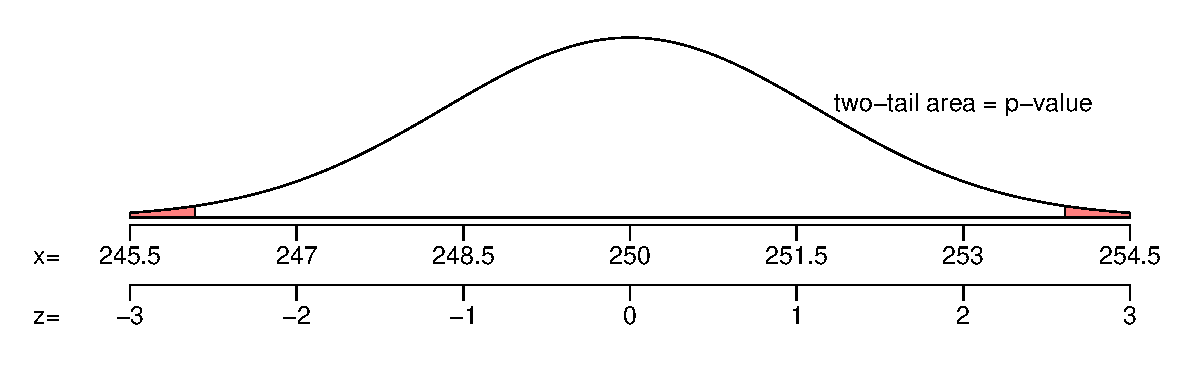
\includegraphics[scale=0.6]{figures/sketch14.pdf}
\end{center}
\end{solution}
\vfill
\part Find a $z$ score of the sample mean.
\begin{solution}
$$z = \frac{253.92-250}{1.5} = 2.61 $$
\end{solution}
\vfill
\part Calculate the $p$-value.
\begin{solution}
$$p\text{-value} ~=~ 2\cdot\Phi(-2.61) ~=~ (2)(0.0045) ~=~ 0.009 $$
\end{solution}
\vfill
\part Make your conclusion.
\begin{solution}
We reject the null hypothesis because $0.009 < 0.01$.
\end{solution}
\vfill
\end{parts}


\newpage

\end{questions}





%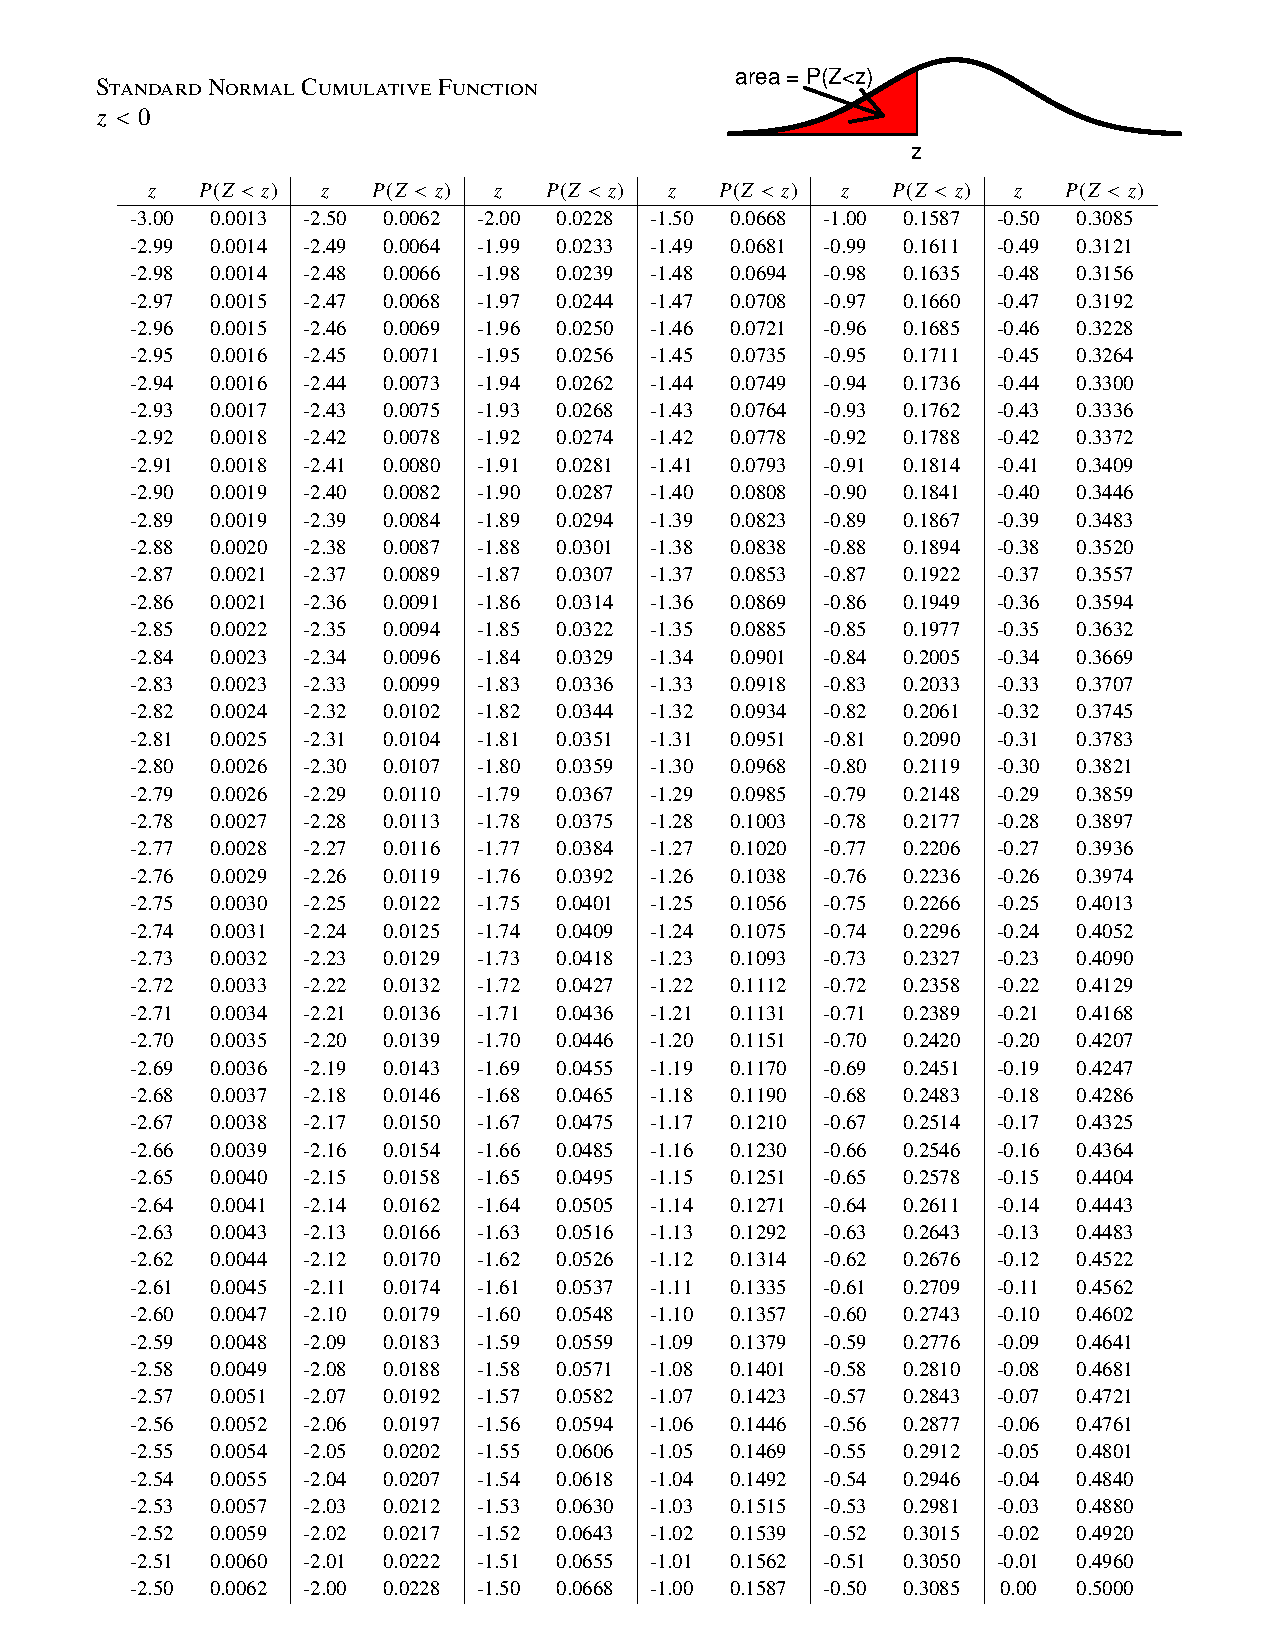
\includepdf[pages=1]{ztable/ztable.pdf}
%\includepdf[pages=2]{ztable/ztable.pdf}

\end{document}
